
\documentclass[11pt]{amsbook}

\usepackage{../HBSuerDemir}	% ------------------------


\begin{document}

% ++++++++++++++++++++++++++++++++++++++
\hPage{b2p1/033}
% ++++++++++++++++++++++++++++++++++++++

\begin{enumerate}[label=(\alph*)]
	\setcounter{enumi}{1}

	\item discuss the convergence and find t as a ratio of two\\
	integers.

\end{enumerate}

\underline{Solution}.

\begin{enumerate}[label=(\alph*)]

	\item $t = 2+\frac{1}{10}+\frac{37}{1000}+\frac{37}{100000}+\ ...\ +\frac{37}{1000.100^{n-1}}+\ ...$\\
	=$\frac{21}{10}+\frac{37}{1000}(1+\frac{1}{100}+\ ...\ +\frac{1}{100^{n-1}}+\ ...)$

	\item The series within the paranthesis is a geometric series\\
	with r = 1/100 which is absolutely less than 1. Then\\
	it is convergent:\\
	$t=\frac{21}{10}+\frac{37}{1000}\frac{1}{1-\frac{1}{100}}=\frac{21}{10}+\frac{37}{990}=\frac{2116}{990} \in \mathbb{Q}$

\end{enumerate}

\begin{exmp} Find the sums:\\
\begin{enumerate}[label=(\alph*)]

	\item $\frac{1}{1.2}+\frac{1}{2.3}+\ ...\ +\frac{1}{n(n+1)}+\ ...$
	
	\item $\frac{1}{2^{2}-1}+\frac{1}{4^{2}-1}+\ ...\ +\frac{1}{(2n)^{2}-1}+\ ...$

\end{enumerate}
\end{exmp}

\underline{Solution}.

\begin{enumerate}[label=(\alph*)]
	
	\item $a_{n}=\frac{1}{n(n+1)}=\frac{A}{n}+\frac{B}{n+1}\Longrightarrow\ A\ =\ 1,\ B\ =\ -1$\par
	$\Longrightarrow a_{n}=\frac{1}{n}-\frac{1}{n+1}$\par
	$\Longrightarrow s_{n}=(1-\frac{1}{2})+(\frac{1}{2}-\frac{1}{3})+\ ...\ +(\frac{1}{n}-\frac{1}{n+1})$\par
	$=1-\frac{1}{n+1}\Longrightarrow S\ =\ 1$
	
	\item $a_{n}=\frac{1}{(2n)^{2}-1}=\frac{A}{2n-1}+\frac{B}{2n+1}\Longrightarrow A=\frac{1}{2},\ B = -\frac{1}{2}$\par
	$\Longrightarrow a_{n}=\frac{1}{2}(\frac{1}{2n-1}-\frac{1}{2n+1})$

\end{enumerate}



% =======================================================
\end{document}  

%==== templates ====

%==== environments ====

%\begin{figure}[htb]
%	\centering
%	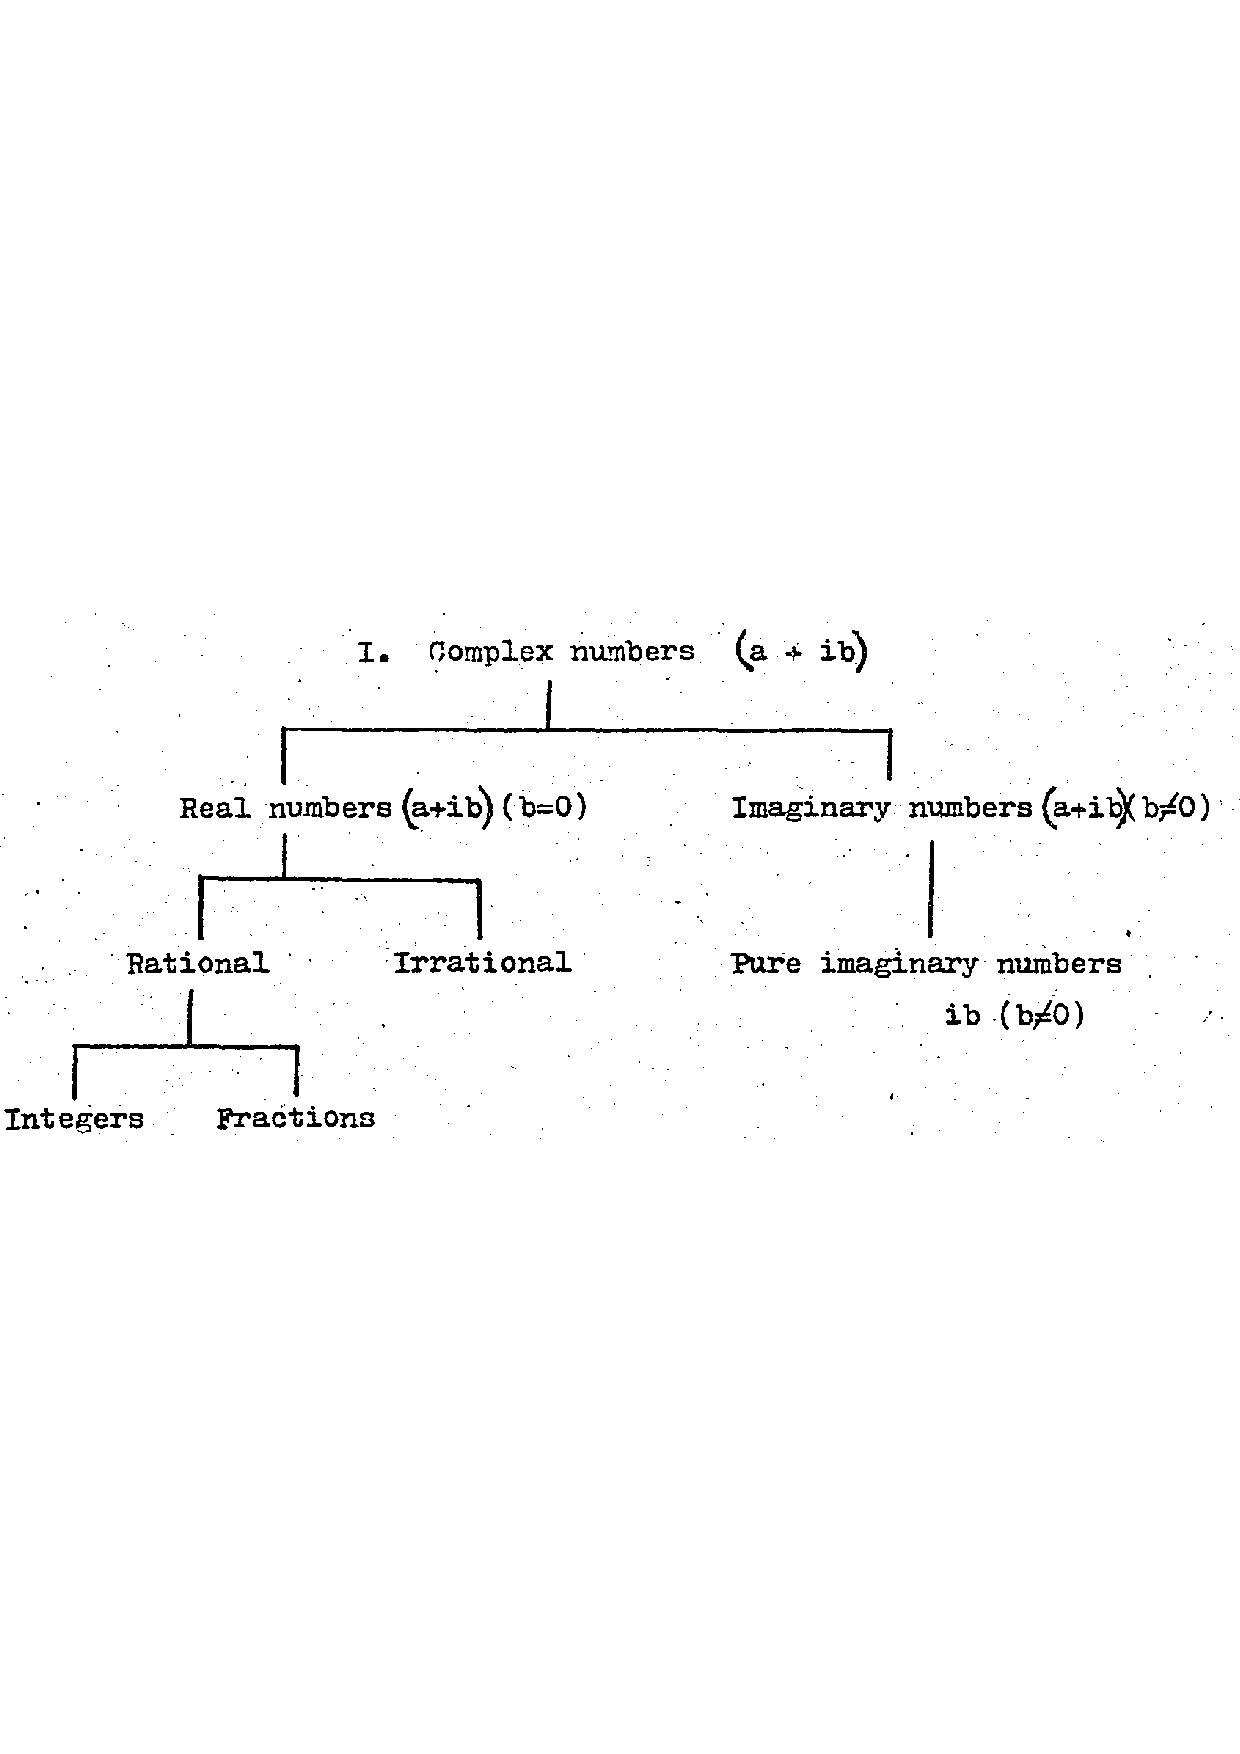
\includegraphics[width=0.9\textwidth]{images/SD-1-1p15A}
%	\caption{Classification of complex numbers}
%	\label{fig:classificationOfComplexNumbersA}
%\end{figure}

%\begin{center}
%\begin{tabular}{cc}
%\end{tabular}
%\end{center}

%\begin{exmp}
%\begin{hSolution}
%\end{hSolution}
%\end{exmp}

%\begin{hEnumerateAlpha}
%\end{hEnumerateAlpha}

%\begin{hEnumerateRoman}
%\end{hEnumerateRoman}

%$
%\begin{bmatrix}
%\end{bmatrix}
%$

%\frac{aaaa}{bbb}
%\frac{a_{n}}{b_{n}}
%\left( aaaa \right)
%\Longrightarrow

%\begin{multicols}{2}
%	bb
%\columnbreak
%	aa
%\end{multicols}
